\section{Entwicklungsansätze mobiler Anwendungen}
\label{sec:Entwicklungsansaetze}

Bei der Entwicklung von Anwendungen für Mobilgeräte wird meist zwischen den drei grundlegenden Ansätzen \textit{Native}, \textit{Hybrid} und \textit{Web} unterschieden \cite{Nunkesser_Taxonomy_Apps, Que_Comparison_Hybrid_Native}.
Die native Entwicklung beschreibt dabei die Anwendungsentwicklung spezifisch für ein bestimmtes Betriebssystem mit den \acp{SDK} und Programmiersprachen, die der Betriebssystemhersteller für die Entwicklung bereitstellt.
Für iOS sind das die Programmiersprachen Objective-C und Swift.
Bei Android kommen Java und Kotlin zum Einsatz.
Sollen beide Betriebssysteme unterstützt werden, muss die Anwendung für jedes System in einer der entsprechenden Sprachen gesondert entwickelt werden.
Für die Entwicklung wird dementsprechend ein Team mit Kenntnissen in beiden Systemen oder getrennte Entwicklungsteams pro Plattform benötigt.
Das hat nicht nur Auswirkungen auf die Entwicklungskosten, sondern auch auf die Geschwindigkeit der Entwicklung \cite{Manchanda_CrossPlatformFrameworks}.
Dennoch wird dieser Ansatz häufig eingesetzt, um die größtmögliche Performance zu erhalten und auf alle vom Betriebssystem zur Verfügung gestellten \acp{API} zugreifen zu können \cite{Pinto_Native_to_Cross_Platform}.

Beim Web-Ansatz hingegen, wird eine einzelne Webanwendung bereitgestellt, die komplett im Browser und damit unabhängig vom Betriebssystem lauffähig ist.
Sie können nicht nur auf Mobilgeräten, sondern auch auf klassischen Desktop-Systemen ausgeführt werden.
Für die Entwicklung von Web-Apps werden klassischerweise \ac{HTML}, \ac{CSS} und JavaScript verwendet.
Verschiedene \ac{CSS}-Bibliotheken unterstützen bei der Umsetzung eines responsiven Designs und können so ein \ac{UI} realisieren, das sowohl auf Desktop-PCs als auch auf Mobilgeräten nutzbar ist.
Darüber hinaus können verschiedene Frontend-Frameworks und Bibliotheken eingesetzt werden, um die Entwicklung von Web-Apps für Mobilgeräte weiter zu vereinfachen.
Beispiele dafür sind Angular oder React, die es ermöglichen Single-Page-Anwendungen zu erstellen, die sich auf Mobilgeräten ähnlich bedienen lassen wie Native-Apps \cite{Pinto_Native_to_Cross_Platform}.
Darüber hinaus bietet der Web-Ansatz weitere Vorteile. 
Unter anderem ist das Deployment neuer Versionen deutlich einfacher, da keine Abhängigkeit zu den jeweiligen App-Stores besteht.
Web Anwendungen haben allerdings die Einschränkung, dass nur Gerätefunktionen die im Browser zur Verfügung stehen genutzt werden können. 
Zugriff auf die \acp{API} des Betriebssystems ist nicht möglich.
Der hybride Ansatz versucht beide Ansätze zu kombinieren, indem Webanwendungen in native Anwendungen eingebettet werden.
Somit können teilweise native Funktionen wie Smartphone-Sensoren und spezielle \acp{API} verwendet werden, während die Anwendung in einem eingebetteten Browser läuft und überwiegend mit Web-Technologien entwickelt werden kann \cite{Nunkesser_Taxonomy_Apps}.

Eine weitere Entwicklung im Bereich der Web-Apps sind \acp{PWA}, welche ähnlich wie hybride Apps teilweise komplett offline genutzt werden können und wie lokal installierte Apps wirken können, aber komplett mit Web-Technologien implementiert werden können \cite{PWA}.
Trotzdem können viele Anwendungsfälle aufgrund von schlechter Performance oder stark eingeschränktem Zugriff auf Hardware und Geräte-\acp{API} nicht zufriedenstellend mit Web-Apps realisiert werden \cite{Pinto_Native_to_Cross_Platform}.


Sowohl hybride als auch Web-Apps ermöglichen die Wiederverwendung von Code zwischen den verschiedenen Plattformen.
Demnach können beide unter dem Überbegriff Cross-Plattform Apps zusammengefasst werden.
Allerdings bieten Web-Apps nur sehr geringen Zugriff auf die Hardware des Geräts und können daher nicht alle Anwendungsfälle abdecken und nicht über die App-Stores der Betriebssysteme verteilt werden.
Deshalb wird bei der Betrachtung von Frameworks für die Plattformübergreifende Entwicklung nicht auf Frameworks für die reine Web-Entwicklung eingegangen.
Stattdessen wird der Fokus auf Frameworks gelegt, die den Zugriff auf Gerätefunktionen ermöglichen und als installierbare App auch über die App-Stores der Betriebssysteme verteilt werden können.

Inzwischen gibt es eine Vielzahl von Frameworks, welche diese Kriterien erfüllen, aber nicht dem hybriden Ansatz zugeordnet werden können.
Deshalb führt Nunkesser in \cite{Nunkesser_Taxonomy_Apps} eine feinere Unterteilung der Entwicklungsansätze auf Basis der verwendeten Tools und Technologien ein.
Die Unterteilung in sechs Kategorien und ihre wichtigsten Merkmale ist in der Tabelle in \ref{tab:Nunkesser_App_Categories} dargestellt.
Außerdem ist in der letzten Spalte angegeben, ob die App-Kategorie die plattformübergreifende Wiederverwendung von Code unterstützt.
\begin{table}[H]
    \begin{tabularx}{\textwidth}{ lXr }
        \textbf{Kategorie}      & \textbf{Kennzeichen}  & \textbf{Plattformübergreifende} \\ & & \textbf{Code-Wiederverwendung}                                                   \\
        \toprule[0.1em]
        Endemic Apps            & Verwendung Plattformspezifischer Tools, \acp{SDK} und Programmiersprachen bereitgestellt vom Betriebssystemhersteller, Kompilation, Teilweise \ac{JIT}-Kompilation möglich                        & \xmark        \\
        \hline
        Web-Apps                & Verwendung von Web-Technologien, Interpretation im Browser des Zielgeräts                                                                                                                         & \cmark        \\
        \hline
        Hybrid Web-Apps         & Verwendung von Web-Technologien, eingebettet in eine Endemic App, Kombination von kompilierten und interpretierten Teilen                                                                         & \cmark        \\
        \hline
        Hybrid Bridged Apps     & Erweiterung von Hybrid Web-Apps um \ac{UI} Elemente von Endemic Apps, Kombination von kompilierten und interpretierten Teilen                                                                     & \cmark        \\
        \hline
        System Language Apps    & Verwendung von Low-Level Programmiersprachen wie C/C++ und Plattformspezifische Kompilation                                                                                                       & (\xmark)      \\
        \hline
        Foreign Language Apps   & Verwendung von Programmiersprachen, die vom Betriebssystemhersteller nicht für Endemic Apps vorgesehen sind, in der Regel Kompilation, Teilweise \ac{JIT}-Kompilation und Interpretation möglich   & \cmark       \\
    \end{tabularx}
    \caption{App-Kategorien und Entwicklungsansätze nach Nunkesser \cite{Nunkesser_Taxonomy_Apps}}
    \label{tab:Nunkesser_App_Categories}
\end{table}

Eine wichtige Neuerung ist die Einführung der neuen Kategorie der \textit{Foreign Language Apps}, welche keiner anderen Kategorie untergeordnet werden können.
Populäre Frameworks wie Xamarin und Flutter gehören zu dieser Kategorie und ermöglichen die Entwicklung mit C\# respektive Dart, welche weder von Android noch von iOS für die Entwicklung von Apps vorgesehen sind \cite{Xamarin_Einfuehrung} \cite{Fentaw_Thesis_Flutter}.
Weiterhin differenziert er den Hybrid Ansatz weiter und führt die Endemic Apps, abgeleitet aus dem griechischen, als neue Bezeichnung für den nativen Ansatz ein.
Alle nicht den Endemic Apps zugeordneten Ansätze nennt er als Gegensatz zu Endemic Apps, Ecdemic Apps.
Außerdem führt er Pandemic Apps als Überbegriff für die Apps, die auf Sprachen setzen die auf beiden Systemen verfügbar sind, wie zum Beispiel C/C++ oder JavaScript \cite{Nunkesser_Taxonomy_Apps}.
Pandemic und Ecdemic dienen vor allem als Überbegriffe zur Sammlung verwandter Ansätze, werden im Folgenden allerdings nicht weiter verwendet.
Nunkessers Taxonomie bietet allerdings auch Bezeichnungen für die einzelnen Ansätze, die das Grundkonzept des jeweiligen Ansatzes einfach verständlich machen.
Deshalb werden die von ihm eingeführten Bezeichnungen im Folgenden verwendet.
Die hierarchische Taxonomie Nunkessers ist in \autoref{fig:Nunkesser_Hierarchy} dargestellt.

\begin{figure}
    \centering
    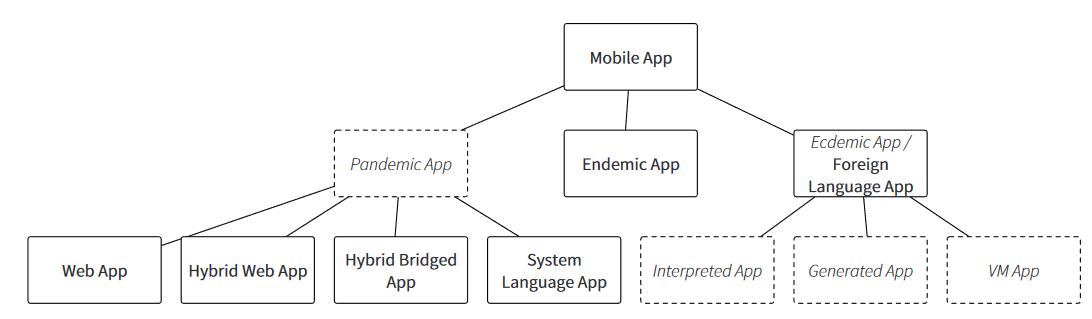
\includegraphics[width=0.9\textwidth]{Nunkesser_Hierarchy.png}
    \caption{Hierarchische Taxonomie der Entwicklungsansätze mobiler Apps \cite{Nunkesser_Taxonomy_Apps}.}
    \label{fig:Native_vs_CrossPlatform}
\end{figure}

Für den Zweck dieser Arbeit wird in den folgenden Abschnitten vorwiegend die übergreifende Kategorie der der Cross-Plattform Apps verwendet.
Diese umfasst die \textit{Hybrid Web Apps}, \textit{Hybrid Bridged Apps} und Foreign Language Apps.
Demnach wird im Folgenden zwischen Native-Apps beziehungsweise Endemic Apps, Web-Apps und Cross-Plattform Apps unterschieden.
Bei der Erläuterung der verschiedenen Frameworks wird dennoch eine Einordnung des jeweiligen Frameworks in eine Kategorie, wie von Nunkesser definiert, vorgenommen.
So können Vergleiche nicht nur zwischen einzelnen Frameworks, sondern auch zwischen verschiedenen Kategorien durchgeführt werden.
Die von Nunkesser als \textit{System Language Apps} bezeichnete Kategorie wird im Rahmen dieser Arbeit nicht zur Cross-Plattform Kategorie zugeordnet.
Bei System Language Apps erfolgt eine starke Bindung an das jeweilige \ac{SDK}, was die Wiederverwendung von Code sehr schwierig macht.
Bei geeigneter Architektur der App ist es hier jedoch möglich, Teile des Codes Systemübergreifend zu verwenden.
Für die Untersuchung von Frameworks für die Plattformübergreifende Entwicklung spielt dieser Ansatz aufgrund fehlender populärer Frameworks keine Rolle.
Außerdem ist die Bedeutung dieses Ansatzes für die Entwicklung mobiler Anwendungen in der Praxis allgemein vergleichsweise gering \cite{Nunkesser_Taxonomy_Apps}.

Obwohl sich die Ansätze der verschiedenen Kategorien, die hier als Cross-Plattform zusammengefasst werden, stark voneinander unterscheiden, weisen sie dennoch genügend Gemeinsamkeiten auf, die diese Zusammenfassung rechtfertigen.
Im Folgenden soll die Bezeichnung Cross-Plattform, jeweils als ein Ansatz verstanden werden, der die Wiederverwendung von Code, insbesondere zwischen den beiden mobilen Plattformen Android und iOS, fördert.
Gefordert wird zusätzlich die Möglichkeit, auf native Gerätefunktionen, wie Gerätesensoren oder die Kamera, zuzugreifen.
Es wird für die Kategorisierung nicht gefordert, dass der komplette Code wiederverwendet werden kann.


\subsection{Vorteile von Cross-Plattform Entwicklung}
\label{sec:CrossPlattform_Vorteile}

Trotz der Unterschiede der verschiedenen Cross-Pattform Ansätze und einzelnen Frameworks, welche im Verlauf dieser Arbeit noch aufgezeigt werden, können einige gemeinsame Vor- und Nachteile des Cross-Plattform Ansatzes identifiziert werden.
Die wichtigsten Vorteile und auch Nachteile der Cross-Plattform Entwicklung im Vergleich zur nativen Entwicklung sind in \autoref{fig:Native_vs_CrossPlatform} tabellarisch aufgeführt.
\begin{figure}[H]
    \centering
    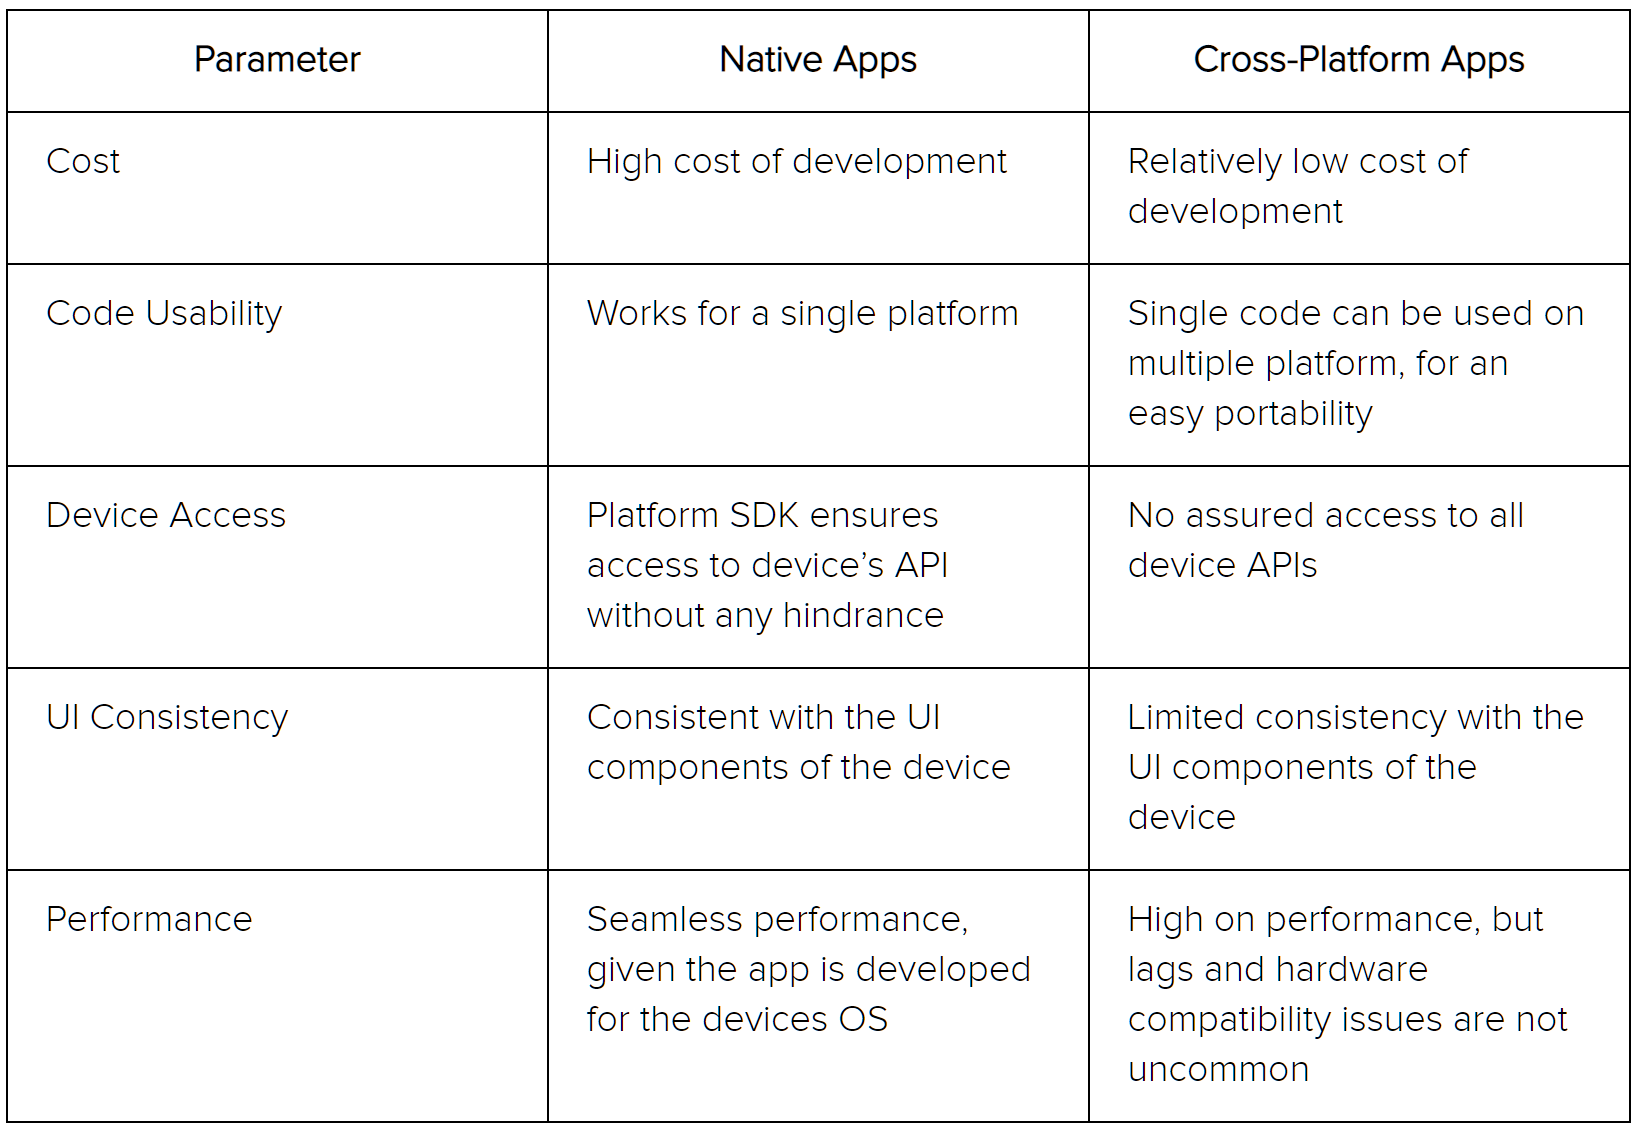
\includegraphics[width=0.9\textwidth]{Native_vs_CrossPlatform.png}
    \caption{Gegenüberstellung Entwicklungsansätze Native und Cross-Plattform \cite{Manchanda_CrossPlatformFrameworks}.}
    \label{fig:Native_vs_CrossPlatform}
\end{figure}

Alle Ansätze der teilen sich den Vorteil eines reduzierten Entwicklungsaufwands durch die einfache Wiederverwendung von Code.
Je nach verwendetem Framework kann der Anteil des geteilten Codes bis zu 100 \% betragen.
Allerdings ist es bei manchen Frameworks notwendig einzelne Funktionen in der jeweils nativen Programmiersprache zu implementieren.
Allgemein kann jedoch der überwiegende Teil des Codes wiederverwendet werden \cite{Nawrocki_Comparison_Hybrid_Native_Frameworks}.
Damit lassen sich die Entwicklungskosten im Vergleich zu nativen Apps durch die Cross-Plattform Entwicklung teils deutlich senken.
Matt Kremer, Enterprise Product Manager für das Ionic-Framework, gibt an, dass bei der Verwendung des Ionic-Frameworks sowohl Zeitaufwände für initiale Entwicklung und spätere Weiterentwicklung als auch die Personalkosten pro Woche geringer sind als bei einer nativen Entwicklung.
In einem Beispiel demonstriert er, wie die Kosten eines Ionic-Projekts weniger als 30 \% der Kosten eines vergleichbaren nativen Projekts betragen können \cite{Kremer_IonicROI}.
Hier ist jedoch zu bedenken, dass diese Angaben nicht durch eine unabhängige Quelle bestätigt wurden.
Dennoch sind sowohl Framework-Entwickler \cite{Xamarin_Einfuehrung, Kremer_IonicROI} als auch unabhängige Literatur \cite{Pinto_Native_to_Cross_Platform, Que_Comparison_Hybrid_Native, Nawrocki_Comparison_Hybrid_Native_Frameworks} einig, dass eine Cross-Plattform Entwicklung Kostenvorteile mit sich bringt.

Allgemeine Probleme gibt es beim Zugriff auf native \acp{API} der Geräte.
Einige Frameworks bieten direkten Zugriff auf einige native \acp{API}, andere setzen für jeglichen Zugriff auf Plugin-Systeme \cite{Heitkoetter_CrossPlatform_Comparison, Sasidaran_Survey_NativeHybrid}.
Meist können in einer Cross-Plattform App jedoch nicht alle nativ zur Verfügung stehenden Schnittstellen verwendet werden \cite{Pinto_Native_to_Cross_Platform}.

Auch bei der Konsistenz der Benutzeroberflächen schneiden die Cross-Plattform Ansätze meist schlechter ab als die native Entwicklung \cite{Manchanda_CrossPlatformFrameworks}.
Allerdings gibt es hier starke Unterschiede zwischen den Frameworks. 
Zum Beispiel verwendet ReactNative jeweils native \ac{UI}-Elemente, sodass die Benutzeroberfläche dem Look-and-Feel der Plattform entspricht \cite{React_NativeComponents}.

Ein gemeinsamer Nachteil aller Cross-Plattform Ansätze ist die durchschnittlich geringere Performance im Vergleich zu nativen Anwendungen \cite{Que_Comparison_Hybrid_Native, Pinto_Native_to_Cross_Platform}.
Einzelne Frameworks können für bestimmte Anwendungszwecke besser geeignet sein und andere können bei Betrachtung anderer Performancemetriken besser abschneiden.
Allgemein ist die Bewertung der Performance eines Frameworks immer vom Anwendungsfall und von der konkreten App abhängig.
In der Literatur finden sich verschiedene Untersuchungen \cite{Nawrocki_Comparison_Hybrid_Native_Frameworks,Biorn-Hansen_PerformanceOverhead_CrossPlatform,Jia_Performance}, welche sich mit der Performance von verschiedenen Cross-Plattform Frameworks beschäftigen. 
In keiner dieser Arbeiten wird jedoch die Performance für den konkreten Anwendungsfall der Videoaufzeichnung ausführlich untersucht.